\chapter{Wireless sensors networks}

Traditional sensor monitoring was implemented with basic sensors made up only by transducers connected by a wire to a centralized device, such as Arduino.
In WSNs instead, the sensors are connected wirelessly to a centralized device, which is usually a computer or a microcontroller, and they present many characteristics:
\begin{itemize}
   \item Intelligent
   \item Wireless
   \item Autonomous
   \item Capable of building a Network
\end{itemize}

\section{Deploying a WSN}

\begin{paracol}{2}
   

   Sensor deployed in a ``Sensing Field'' form a network made up ---one or more--- sink nodes and a set of sensor nodes.
   Each sensor produces a stream of data which may be preprocessed by the sensor itself before being eventually sent to a sink node.
   Sinks may not always be available, so the sensors may act as ``loggers'' and store data for future retrieval; since energy efficiency is a key factor, some \textbf{data aggregation} may be performed on the network to improve the efficiency.
   
   \switchcolumn
   \begin{figure}[htbp]
      \centering
      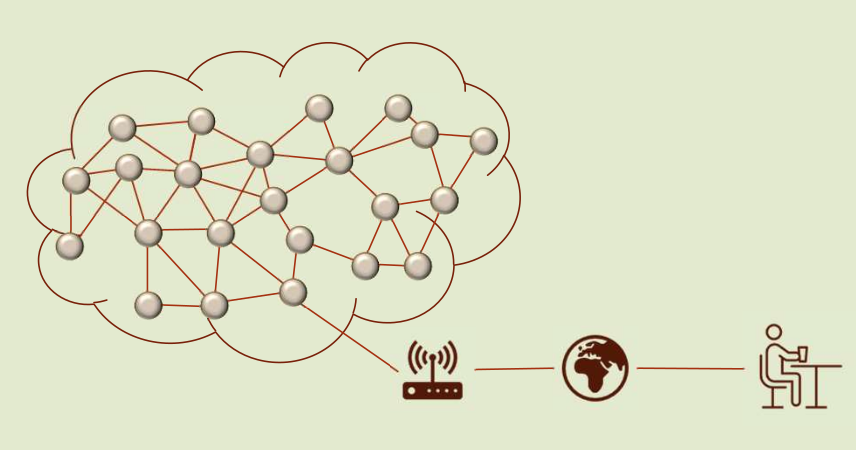
\includegraphics{images/wsn_arch.png}
      \caption{WSN architecture}
      \label{fig:wsn_arch}
   \end{figure}
\end{paracol}

\subsection{WSNs Strenghts}
\begin{paracol}{2}
   \begin{itemize}
      \item Network deployment is easy:
      \begin{itemize}
         \item no need for cables
         \item self-configurable (no centralized control)
   \end{itemize}
   \item Sensors are cheap:
   \begin{itemize}
      \item The number of sensors can scale up
      \item redundant sensors to enforce fault tolerance
   \end{itemize}
   \item Sensors can be mobile
   \begin{itemize}
      \item if wearable or deployed on mobile objects
   \end{itemize}
   \item Sensors can be programmable on the fly
   \begin{itemize}
      \item to adapt to changing conditions
      \item to implement new sensing tasks
   \end{itemize}
\end{itemize}
\switchcolumn
\begin{figure}[htbp]
   \centering
   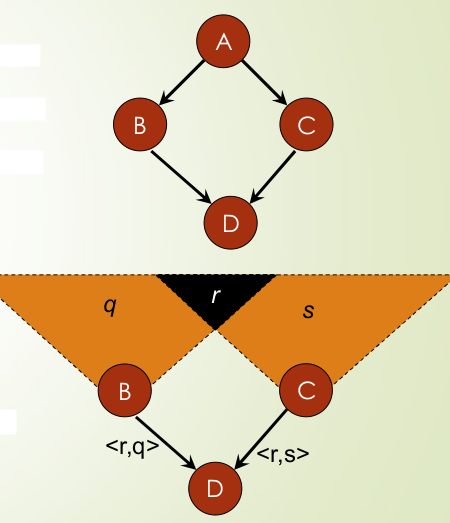
\includegraphics{images/wsn_implosionoverlap.png}
   \caption{Implosion and Overlap issues, described in Sec. \ref{sec:implosionoverlap}}
   \label{fig:wsn_implosionoverlap}
\end{figure}
\end{paracol}

\section{WSN Characteristics}
WSNs first of all may be data-centric or node-centric. This refers especially to routing algorithms, since tradinational ones are too resource-consuming for WSNs.
Most WSN are data-centric, meaning that the data is the most important thing, and the network is built around it.

\subsection{Implosion and Overlap}
\label{sec:implosionoverlap}
The \textbf{``implosion''} problem happens due to flooding-based dissemination:
\begin{itemize}
   \item node A starts by flooding its data to all of its neighbors, including B,C connected to node D.
   \item Two copies of the data eventually arrive at
   the aggregation node D.
   \item The system wastes resources in one
   unnecessary send and receive.
\end{itemize}

The \textbf{``overlap''} problem happens when two nodes send the same data to the same node, which is a waste of resources. 
This may happen when to sensor cover the same overlapping geographical region, (e.g. two cameras covering the same area, or two termometers in the same room) in Figure \ref{fig:wsn_implosionoverlap}, such region is the \textit{``r''} marked.

\subsection{Directed Diffusion}
This is an approach designed and presented by \textbf{Deborah Estrin} and her team in 2000 at Mobicom.

\begin{itemize}
   \item Data is \textbf{named} using attribute-value pairs.
   \item The sink disseminates a sensing task in the network as an interest for named data.
   \item The dissemination of interests sets up gradients.
   \item \note{gradients ``draw'' events (i.e. data matching the interest)}
   \item Data matching the interest flows towards the sink
   \note{Along the gradients, following multiple paths}
   \item The sink \textit{reinforces} one or some of these paths.
\end{itemize}

% Interest ::= <name, attribute-value pairs>
% Data ::= <name, attribute-value pairs>
% Gradient ::= <name, attribute-value pairs>
{\ns\ul{Interest are named by a sequence of attribute-value pairs that describe the task}.
\begin{lstlisting}
   type        = four-legged animal       // detect animal location
   interval    = 20 ms                    // send back events every 20 ms
   duration    = 10 seconds               // .. for the next 10 seconds
   region      = [-100, 100, 200, 400]    // from sensors within rectangle
\end{lstlisting}}
{\ns The data sent in response to the interest is also named using a similar naming scheme.
\begin{lstlisting}
   type        = four-legged animal       // type of animal seen
   instance    = elephant                 // instance of this type
   location    = [125, 220]               // node location
   intensity   = 0.6                      // signal amplitude
   confidence  = 0.85                     // confidence in the match
   timestamp   = 01:20:40                 // event generation time
\end{lstlisting}}

An interest is associated to a duty cycle (?), which is the time interval between two consecutive transmissions of the same interest. \ul{\textit{``Refreshes''}} (i.e. broadcasting again the same interest) are necessary because dissemination of interests is not reliable.
The \ul{first broadcast} of an interest instead is called \ul{\textit{``Exploratory''}}.

Nodes \textbf{cache} the received interests, allowing for ones differing only for sampling rate to be aggregated; interests in cache expire when the duration time expires.\\
Each interest in cache has a \textbf{gradient}, which expresses:
\begin{itemize}
   \item a direction (the node from which the interest was received), used to route data back to the sink
   \item a data rate
\end{itemize}

\section{Direct Diffusion Finite State Machine}
\begin{figure}[htbp]
   \centering
   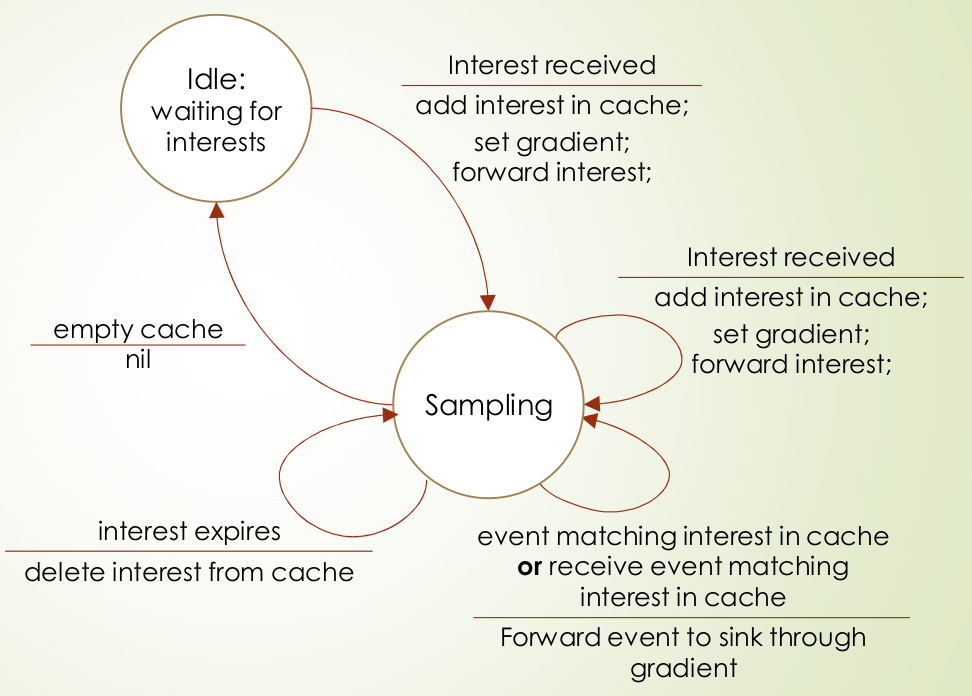
\includegraphics{images/ddiff_FSM.png}
   \caption{Direct Diffusion Finite State Machine}
   \label{fig:ddiff_FSM}
\end{figure}
When a sensor detects an event matching with an interest in
cache:
\begin{enumerate}
   \item  Starts sampling the event at the largest sampling rate of the corresponding gradients
   \item Sends sampled events through the gradients associated to the interests in cache
   \item[-] These gradients correspond to the neighbors interested in the event
\end{enumerate}
Neighbors forward the data only if a corresponding interest (with a gradient) is in their cache, and if the data has not been forwarded before (i.e. redundant copies are dropped).

\begin{paracol}{2}
   \colfill
   Once it has received data matching an exploratory interest from sensor $n$, the sink reinforces $n$ to improve the quality (higher sampling rate) of received data
   \begin{itemize}
      \item Exploratory interests usually have a low sampling rate
      \item Reinforces of interests specify an interest with \textit{higher sampling rate}
      \item In turn, the reinforce propagates along the path from which the events are received up to sensor $n$
   \end{itemize}
   The \textit{overlap} problem instead (multiple sensors covering the same area) is not addressed by this approach, and may still occur(?).\\
   \ul{\textbf{Reliability} is \textit{not} guaranteed}, since a message may be lost, however, it's not a big deal, there will soon be another one \smiley.
   \colfill
   \switchcolumn
   \begin{figure}[htbp]
   \centering
   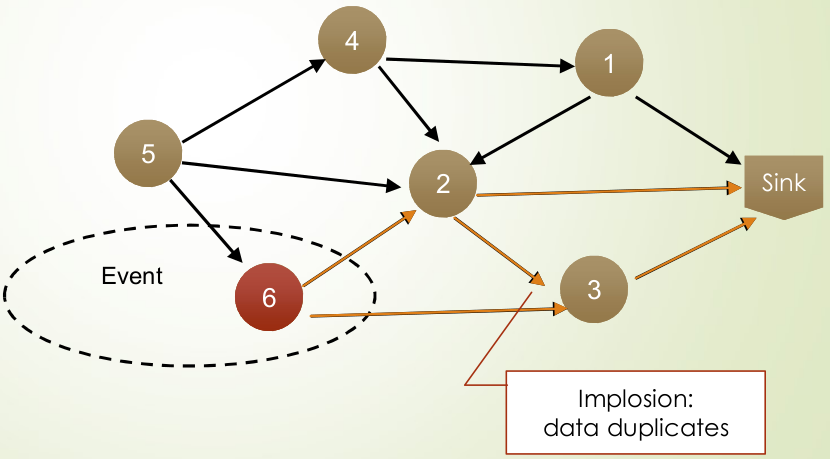
\includegraphics{images/wsn_ddiff_implosion.png}\\
   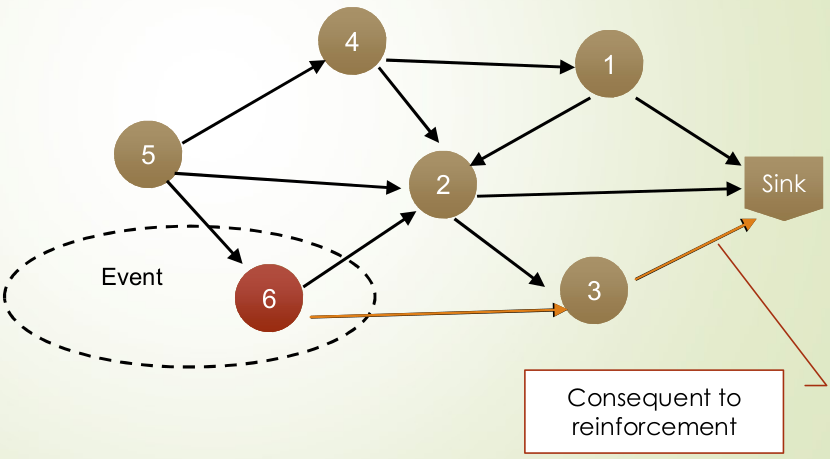
\includegraphics{images/wsn_ddiff_reinforcement.png}
   \caption{Since the gradients ---routes to the sink--- may be multiple, \textit{implosion} may occur. The sink, once it has received data from a sensor $n$, may reinforce one of the paths to avoid this.}
   \label{fig:wsn_ddiff_reinforcement}
   \end{figure}
\end{paracol}

\framedt{
   Assumptions
}{
   Note that Direct Diffusion works under the following key assumptions:
   \begin{itemize}
      \item One sink (with \texttt{id 0} and denoted $n_0$)
      \item the sink has a double radio interface: one to the WSN and one
      to the internet
      \item Each node has a unique \texttt{id} (denoted $n_i$)
      \item The sink initializes and maintains the routing tree
      \item Unicast messages from sensors to the sink
      \item Only the sink broadcasts to the entire network
      \item Sink has 2 antennas: one for the WSN and one for the internet
      \end{itemize}}
\newpage


\section{Topologies}

\begin{paracol}{2}
   \colfill
   Trees provide scalability but sink nodes (two corners of the figure) have larger power consumption, just as nodes close to them, which act as \textbf{bottlenecks}.
   Note that the position in the tree resembles the phyisical position of the nodes in the field, which is often not arbitrary, but is dictated by various factors instead.   
   \colfill
   \switchcolumn
   \begin{figure}[htbp]
      \centering
      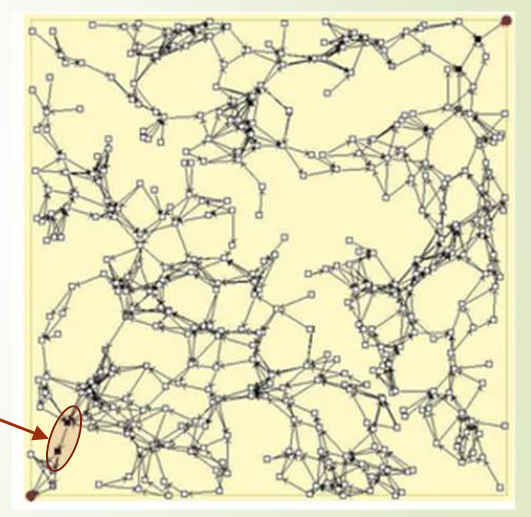
\includegraphics{images/ddiff_trees.png}
      \caption{WSN Tree topology issue}
      \label{fig:ddiff_trees}
   \end{figure}
\end{paracol}

There some major drawbacks for WSN in tree topologies:
\begin{enumerate}
   \item Sink must always be connected to the network (which in turn is not autonomous) 
   \item Does not exploit ---even if little--- processing and storage capabilities of the sensors
   \item Detection of composite events requires communication among sensors
   \item Bottlenecks and load unbalance
\end{enumerate}

On the other side, without trees we need more complex routing algorithms, which are more resource-consuming. That's where GPSR comes in.

\section{GPSR}
The desire was to provide internet-like routing, but without the resource overhead of traditional routing algorithms, in order to overcome the drawbacks of WSN applied to tree topologies.
This problem was addressed in 2003 by \textbf{Brad Karp} and \textbf{H. T. Kung} with the \textbf{Greedy Perimeter Stateless Routing} algorithm, which exploits the GPS information of the nodes to route the packets.

The protocol works under three assumptions:
\begin{itemize}
   \item The network is \textbf{connected}\\
   Source knows the coordinate of the destination.
   \note{This is kind of odd, since nodes only have a local view of the network, not of the whole network.
   So\dots \textit{how does the source know the destination's coordinates?}
   
   }
   \item The network is \textbf{planar}\\
   Nodes are deployed in a 2D plane, and the network is planar if no two nodes overlap.
   \item The network is \textbf{localized}\\
   Nodes are aware of their own position and of the position of the neighbors
\end{itemize}
The protocol completely removes the need for route discovery and consequent route caches and routing tables.

\newpage
\subsection{Greedy and Perimeter Modes}
\begin{paracol}{2}
   
   GSPR comprises two modes:
   \begin{itemize}
      \item \textbf{Greedy forwarding}\\
      The packet is forwarded to the neighbor that is closest to the destination.\\
      More formally,
      The forwarding node $x$ select as next hop a neighbor $y$ such that $y$ is closer to Destination D than $x$ and that $y$ is the closes to D among all the neighbors of $x$.\\
      Greepy forwarding fails if it encounters a \textit{void} region.
      \item \textbf{Perimeter forwarding}\\
      The packet is forwarded to the neighbor that moves it along the perimeter of the void region.\\
      It is based on the \texttt{LHL} (Left Hand on the Left) rule, or the \texttt{RHR} (Right Hand on the Right) rule; i.e. When arriving from y to x selects the first
      counterclockwise edge from $(x,y)$.\\
      In other words, the packet traverses the interior of a closed polygonal region (face) in clockwise ---or counterclockwise--- order.
   \end{itemize}
   \switchcolumn
   
   \colfill
   \begin{figure}[htbp]
      \centering
      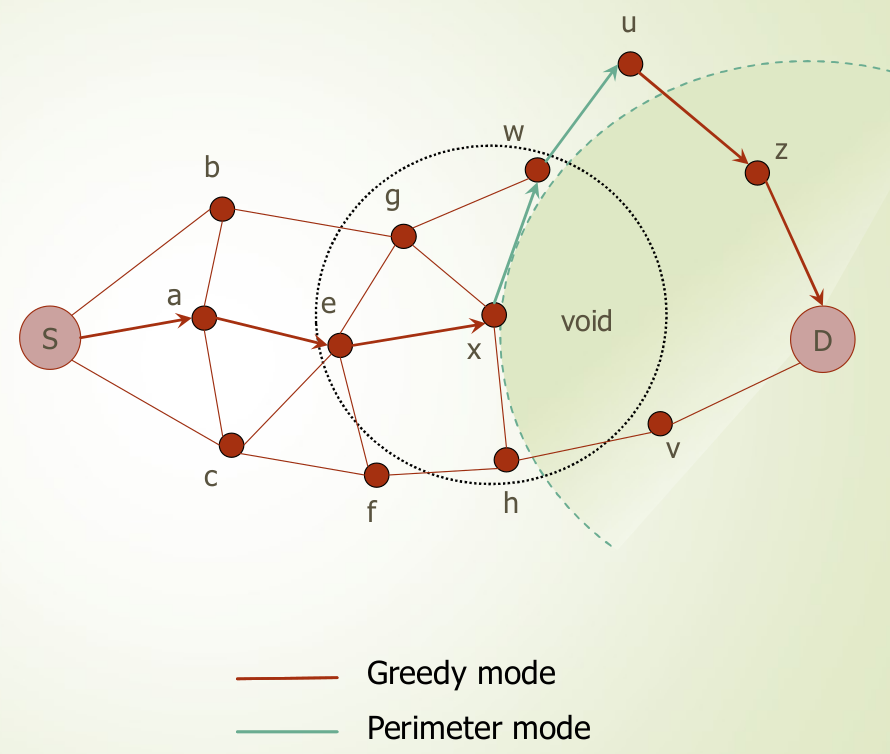
\includegraphics{images/GPSR_modes.png}
      \caption{GPSR Greedy and Perimeter forwarding}
      \label{fig:GPSR_modes}
   \end{figure}
   \colfill

\end{paracol}

\framedt{Switching from the two modes}{
   The switch from Greedy to Perimeter mode is triggered when the Greedy mode fails, i.e. when the node finds a void region, so no nodes closer to $D$ are reachable.\\
   The switch back to Greedy mode cannot be triggered as the node exits the void region, since this may lead to fallback loops.
   The switch is instead performed when a node closer to D than $\tilde{x}$ ---the node from which the perimeter mode started--- is found.
}

\subsection{More on Perimeter mode}
RHR applied to a non-planar graph may lead to a degenerate tour that does not trace the boundary of a closed polygon.
For this reason, given the non-planar graph $G$, the algorithm constructs a planar ---sub---graph $P$ of $G$, and applies RHR to $P$; 
$P$ may either be the
\begin{itemize}
   \item \textit{Relative Neighborhood Graph} of $G$
   \begin{figure}[htbp]
      \centering
      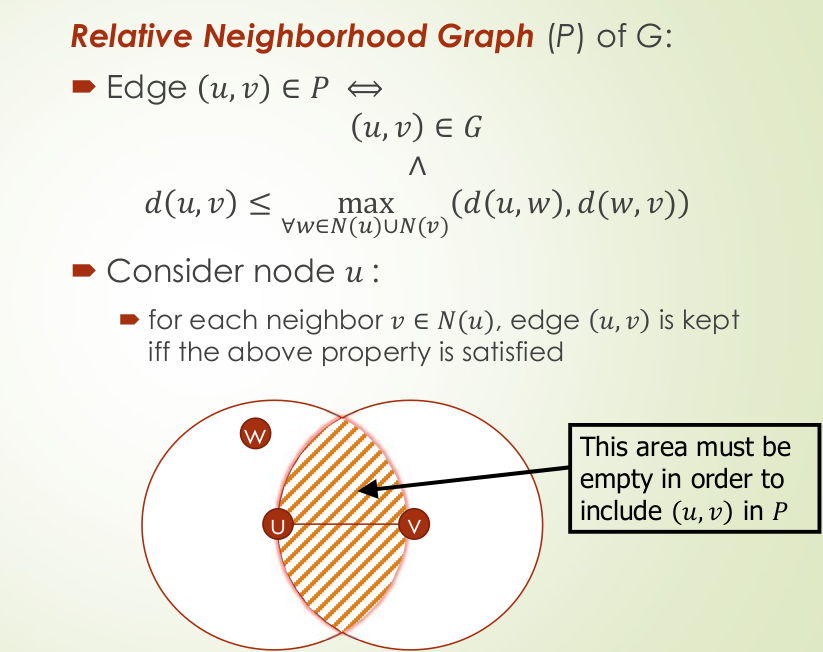
\includegraphics{images/wsn_planarization_1.png}
      % \caption{}
      \label{fig:wsn_planarization_1}
   \end{figure}
   \item \textit{Gabriel Graph} of $G$
   \begin{figure}[htbp]
      \centering
      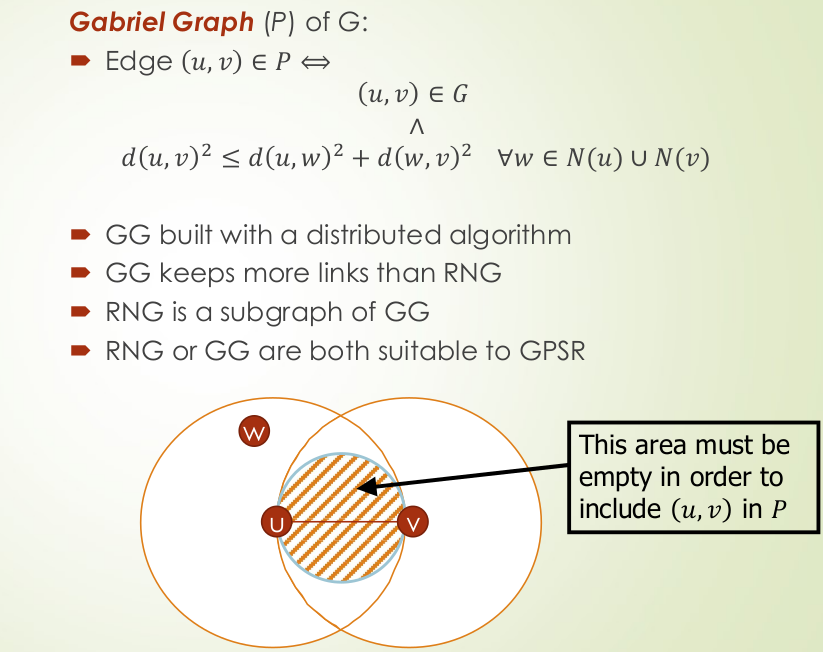
\includegraphics{images/wsn_planarization_2.png}
      % \caption{}
      \label{fig:wsn_planarization_2}
   \end{figure}
   \item[] 
   \begin{figure}[htbp]
      \centering
      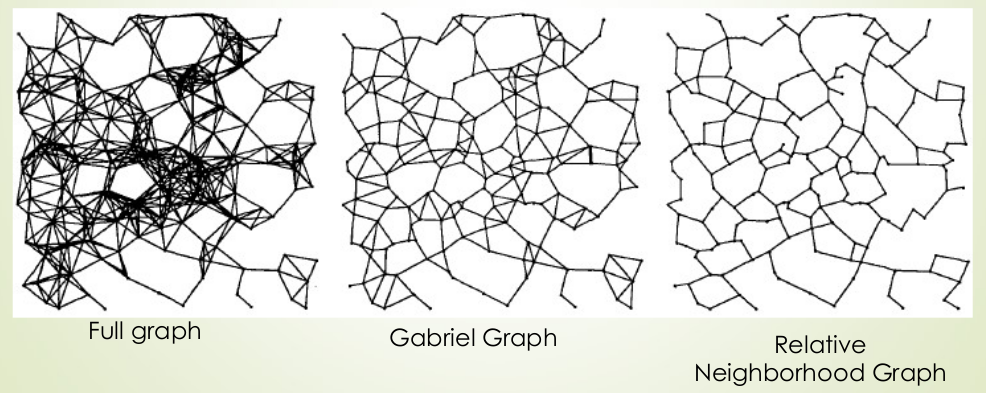
\includegraphics{images/wsn_planarization_3.png}
      % \caption{}
      \label{fig:wsn_planarization_3}
   \end{figure}
\end{itemize}

Greedy mode exploits the whole graph $G$, while Perimeter mode exploits only the links in the planar graph $P$.
\nl

\framedt{Mobility}{
   The problem with GPSR is \textbf{mobility}, mostly due to the need for a planar graph for perimeter mode to work correctly.
   It needs a freshly planarized graph, using ``stale'' planarized graph may result in performance degradation;
   On the other side, planarizing the graph at each topology change is not good either, since it may lead to link instability, because nodes may move within a node’s transmission range, which may continuously change the selection of links by GG or RNG.
   
   To solve the problem, a proactive approach is used, where nodes periodically communicate their position to their neighbors (beaconing), and beacons are used to keep the neighbor’s list.
   When the changes are excessive, planarization is performed.
}
\note{
There are three possible configurations for GPSR responsible for possible loops.
The most problematic is the umbrella-shaped one.
Since the configuration may be complex and made up of multiple nodes, it is not easy to detect, and doing would required the whole view of the network.}

\newpage
\subsection{GPSR obstacle fail}
\begin{figure}[htbp]
   \centering
   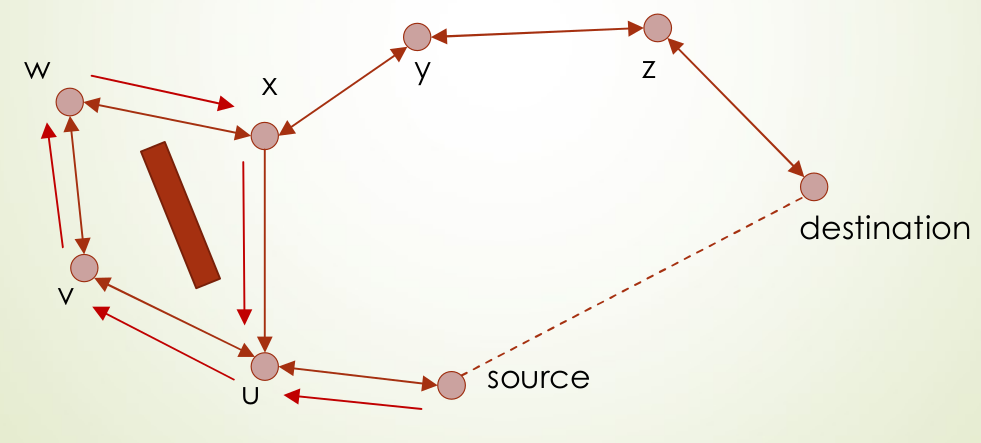
\includegraphics{images/wsn_planarization4.png}
   \caption{Planarization loop with obstacle}
   \label{fig:wsn_planarization4}
\end{figure}
In case of an obstacle, the planarization may lead to a loop, as shown in Figure \ref{fig:wsn_planarization4}.
TODO explain